\newcommand{\graphformatfig}{
\begin{figure}[h]
    \centering
    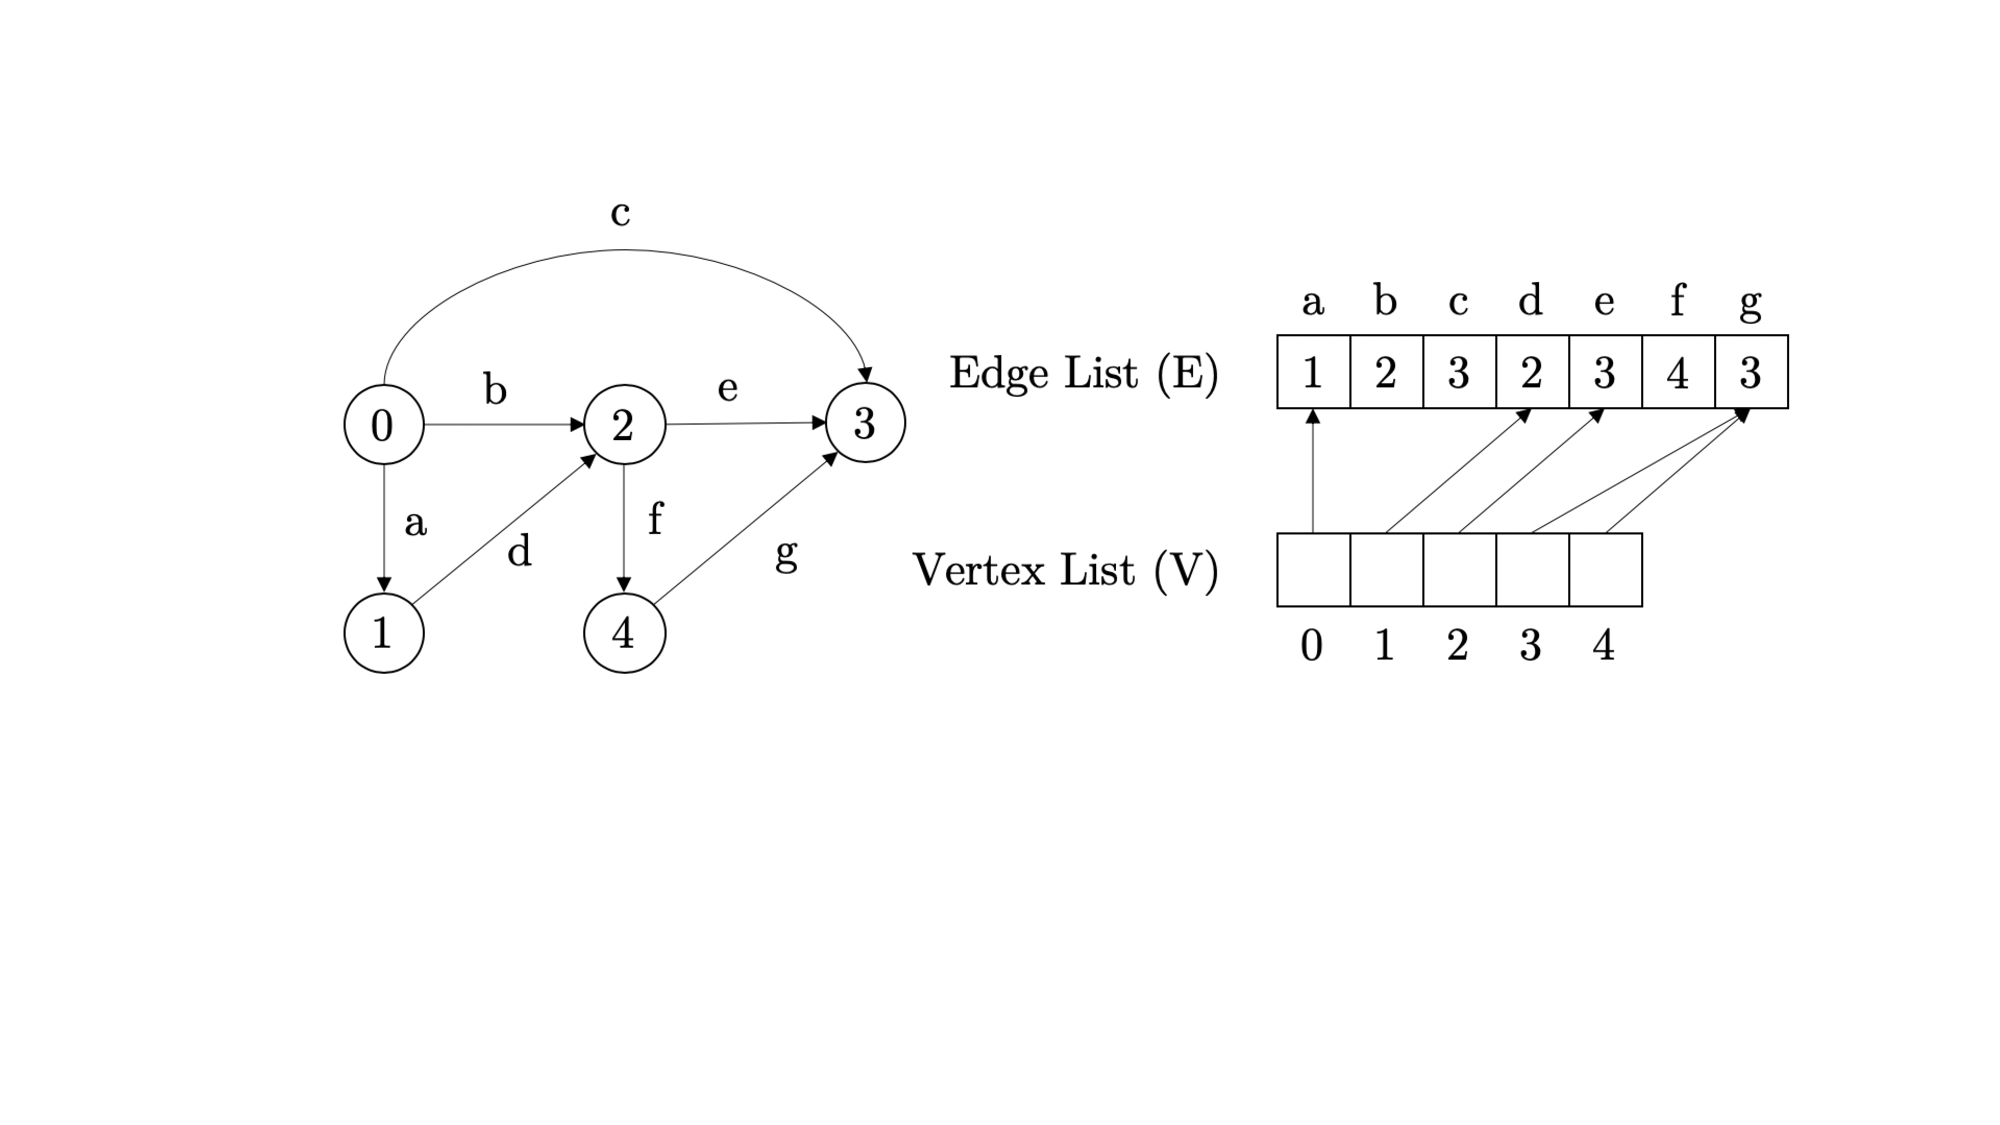
\includegraphics[width=0.8\textwidth]{graphit-figures/graph-format-figure.pdf}
    \caption{The CSR graph format that we use to store graph data on the manycore. For weighted graphs, the weight is stored with each element in the edge array.}
    \label{pap:generals2020:sec:background:fig:graphformat}
\end{figure}
}
\subsection{GraphIt: A Graph Processing Domain-Specific Language}\label{pap:generals2020:sec:graphit}

GraphIt is a domain-specific language for graph processing applications~\citep{zhang2018graphit}.
Like Halide~\citep{ragan2013halide}, GraphIt separates the description of the algorithm from the scheduling of the computation. A separate algorithm language and scheduling language are used to specify graph programs in GraphIt. This separation of description and schedule allows users to express computation more flexibly.
Listing~\ref{pap:generals2020:sec:background:lst:graphit} shows an example GraphIt program implementing Breadth-First Search (BFS).

\begin{lstlisting}[language=graphit, 
                   caption=GraphIt code for Breadth-First Search (BFS),
                   label=pap:generals2020:sec:background:lst:graphit]
const edges : edgeset{Edge}(Vertex,Vertex);
var frontier : vertexset{Vertex} = new vertexset{Vertex}(0);
const parent : vector{Vertex}(int) = -1;

func updateEdge(src : Vertex, dst : Vertex)
    parent[dst] = src;
end

func toFilter(v : Vertex) -> output : bool
    output =  parent[v] == -1;
end

func main()
    // frontier setup
    while (frontier.getVertexSetSize() != 0)
      #s1# frontier = edges.from(frontier).to(toFilter).applyModified(updateEdge,parent,true);
    end
end

schedule:
  program->configApplyDirection("s1", "DensePull")->generateManycoreCode();
\end{lstlisting}

\subsubsection{Graph Representation}
Graphs are represented by \lstinline[language=graphit]{edgeset} and \lstinline[language=graphit]{vertexset} structures.
The edges between nodes are stored as an \lstinline[language=graphit]{edgeset}, and any vertex specific data is stored as a \lstinline[language=graphit]{vertexset}.
Line~1 and Line~2 of Listing~\ref{pap:generals2020:sec:background:lst:graphit} demonstrate the declaration of the \lstinline[language=graphit]{edgeset} variable \lstinline[language=graphit]{edges} and  \lstinline[language=graphit]{vertexset} variable \lstinline[language=graphit]{frontier}. 
Any data associated with elements in an \lstinline[language=graphit]{edgeset} or \lstinline[language=graphit]{vertexset} is stored as a \lstinline[language=graphit]{vector}.
Line~3 of Listing~\ref{pap:generals2020:sec:background:lst:graphit} shows the declaration of a \lstinline[language=graphit]{vector} variable, \lstinline[language=graphit]{parent}, that contains data associated with the vertices in the graph.

GraphIt uses Compressed Sparse Row (CSR) graph format for these data structures, illustrated in Figure~\ref{pap:generals2020:sec:background:fig:graphformat}.
CSR format represents a graph with two arrays: a vertex list and an edge list.
The edge list contains the destination vertex for each edge in the graph and contains $|E|$ elements where $E$ is the set of edges in the graph.
In the case of a weighted graph, the edge list is stored as an array of tuples, with each element in the array containing the destination vertex id and the weight of the edge.
The vertex list contains $|V|$ elements where $V$ is the set of vertices in the graph. 
Each element in the vertex list is an index into the edge list array.
This index corresponds to the start of the edges for which that vertex is the source vertex.
The number of edges for a vertex $v$, or its degree, is $vertex\_list[v+1] - vertex\_list[v]$.
The generated code operates on these arrays to perform computation.

\graphformatfig


\subsubsection{Algorithm Representation}
An algorithm in GraphIt is written as operations on \lstinline[language=graphit]{edgeset} and \lstinline[language=graphit]{vertexset} datatypes. 
Graphit provides several operators that perform computation on these types, but the most common are the \lstinline[language=graphit]{filter} operator and \lstinline[language=graphit]{apply} operator.
The \lstinline[language=graphit]{filter} operator takes a function and a set, applies the function to each element in the set, and returns a set of elements where the function returned true.
The \lstinline[language=graphit]{apply} operator takes a function and set as input and applies the function to each element in the set. %, and returns the resulting set of modified elements.
GraphIt also provides other built-in operators like \lstinline[language=graphit]{applyModified}, that takes a function and a set, applies the function to each element in the set, and returns a vertexset that contains vertices that were updated by the input function. 
This operator is used to construct frontiers in iterative graph algorithms. 
Listing~\ref{pap:generals2020:sec:background:lst:graphit} demonstrates how these operators can be used to write BFS.

Line~16 of Listing~\ref{pap:generals2020:sec:background:lst:graphit} demonstrates two uses of the \lstinline[language=graphit]{filter} operator and one use of the \lstinline[language=graphit]{applyModified} operator. 
The first filter application (\lstinline[language=graphit]{from(frontier)}) selects only edges with source vertices that are in the current frontier. 
The second filter application (\lstinline[language=graphit]{to(toFilter)}) uses the \lstinline[language=graphit]{toFilter} function, defined on line~9, to select edges with destination vertices that haven't been previously visited.
Next, an \lstinline[language=graphit]{applyModified} operator is applied to this filtered set of edges.
This operator computes the edge traversal of BFS and returns a vertexset containing the vertices that were updated by the \lstinline[language=graphit]{updateEdge} function defined on line~5.
This \lstinline[language=graphit]{vertexset} becomes the new frontier for the next iteration of the while-loop.
%\todo[inline]{Check all line-number references}

\subsubsection{Schedule Representation}
GraphIt provides a wide range of scheduling options, i.e., by specifying traversal direction, by specifying the level of parallelism, or by using load balancing techniques for parallel operators.
Labels are used to indicate which operators in the algorithm description the scheduling optimizations should be applied to.
The separation of the algorithm description and schedule allows developers to iterate through different scheduling optimizations and is a key part of GraphIt.
The schedule finishes by generating code for the target device.
The schedule description always follows the algorithm description in GraphIt.

The schedule for BFSs starts with the \lstinline[language=graphit]{schedule} declaration on Line~20 of Listing~\ref{pap:generals2020:sec:background:lst:graphit}. Line~21 specifies that the schedule for label \lstinline[language=graphit]{#s1#} should be "Dense Pull". This schedule is described in Section~\ref{sec:method}
Finally, the schedule specifies that the code generator should generate code for the target device. 

\subsubsection{Code Generation}
GraphIt's code generator takes an algorithm and schedule and generates device-specific code.
Graphit first parses the algorithm and schedule using the frontend to produce the Intermediate Representation. 
Next, the compiler performs dependency analysis and enforces restrictions on read-write accesses and reduction operators. 
Once the compiler verifies the validity of the algorithm and schedule, the backend generates code for the target device and host (if necessary).
%Section~\ref{sec:method} describes how our back end generates manycore code.
